\section{Überschrift}
Lorem ipsum dolor sit amet, consetetur sadipscing elitr, sed
diam nonumy eirmod tempor invidunt ut labore et dolore
magna aliquyam erat, sed diam voluptua. At vero eos et
accusam et justo duo dolores et ea rebum. Stet clita kasd
gubergren, no sea takimata sanctus est Lorem ipsum dolor
sit amet.
\subsection{Unterüberschrift}
Consetetur sadipscing elitr, sed diam nonumy eirmod
tempor invidunt ut labore et dolore magna aliquyam erat,
sed diam voluptua. At vero eos et accusam et justo duo
dolores et ea rebum. Stet clita kasd gubergren, no sea
takimata sanctus est Lorem ipsum dolor sit amet. Lorem
ipsum dolor sit amet, consetetur sadipscing elitr, sed diam
nonumy eirmod tempor invidunt ut labore et dolore magna
aliquyam erat, sed diam voluptua. At vero eos et accusam
et justo duo dolores et ea rebum. Stet clita kasd gubergren,

\section{Überschrift 1}
Lorem ipsum dolor sit amet, consetetur sadipscing elitr, sed
diam nonumy eirmod tempor invidunt ut labore et dolore
magna aliquyam erat, sed diam voluptua. At vero eos et
accusam et justo duo dolores et ea rebum. Stet clita kasd
gubergren, no sea takimata sanctus est Lorem ipsum dolor
sit amet. Lorem ipsum dolor sit amet, consetetur sadipscing
elitr, sed diam nonumy eirmod tempor invidunt ut labore et
dolore magna aliquyam erat, sed diam voluptua. At vero
eos et accusam et justo duo dolores et ea rebum. Stet clita
kasd gubergren, no sea takimata sanctus est Lorem ipsum
dolor sit amet. Lorem ipsum dolor sit amet, consetetur
sadipscing elitr, sed diam nonumy eirmod tempor invidunt
ut labore et dolore magna aliquyam erat, sed diam
voluptua. At vero eos et accusam et justo duo dolores et ea
rebum. Stet clita kasd gubergren, no sea takimata sanctus
est Lorem ipsum dolor sit amet.


%Duis autem vel eum iriure dolor in hendrerit in vulputate
%velit esse molestie consequat, vel illum dolore eu feugiat
%nulla facilisis at vero eros et accumsan et iusto odio
%dignissim qui blandit praesent luptatum zzril delenit augue
%duis dolore te feugait nulla facilisi. Lorem ipsum dolor sit
%amet, consectetuer adipiscing elit, sed diam nonummy nibh
%euismod tincidunt ut laoreet dolore magna aliquam erat volutpat.   


Ut wisi enim ad minim veniam, quis nostrud exerci tation ullamcorper suscipit lobortis nisl ut aliquip ex ea commodo consequat. Duis autem vel eum iriure dolor in hendrerit in vulputate velit esse molestie consequat, vel illum dolore eu feugiat nulla facilisis at vero eros et accumsan et iusto odio dignissim qui blandit praesent luptatum zzril delenit augue duis dolore te feugait nulla facilisi.   


Consetetur sadipscing elitr, sed diam nonumy eirmod tempor invidunt ut labore et dolore magna aliquyam erat, sed diam voluptua. At vero eos et accusam et justo duo dolores et ea rebum. Stet clita kasd gubergren, no sea takimata sanctus est Lorem ipsum dolor sit amet. Lorem ipsum dolor sit amet, consetetur sadipscing elitr, sed diam nonumy eirmod tempor invidunt ut labore et dolore magna aliquyam erat, sed diam voluptua. At vero eos et accusam et justo duo dolores et ea rebum. Stet clita kasd gubergren, no sea takimata sanctus est Lorem ipsum dolor sit amet. Lorem ipsum dolor sit amet, consetetur sadipscing elitr, sed diam nonumy eirmod tempor invidunt ut labore et dolore magna aliquyam erat, sed diam voluptua. At vero eos et accusam et justo duo dolores et ea rebum. Stet clita kasd gubergren, no sea takimata sanctus.  

\section{Umfang der Hausarbeit}
Die Hausarbeit sollte 3-7 Seiten umfassen (in der angegebenen Formatierung, siehe auch (FKT 2019)).
\section{Zitate und Referenzen}
Alle Hausarbeiten müssen den Author/Jahr-Stil verwenden, also z.B. (FKT 2019).
Für die Formatierung ist die Reference-Formatvorlage zu verwenden. Alle Referenzen müssen alphabetisch sortiert sein.

Zitieren der Beispielquelle: \cite{beispiel}

\section{Bilder}
Hier gehts im Bilder.
\subsection{Ein Bild in einer Spalte}
Hier soll ein Bild innerhalb einer Spalte hin.

\par\medskip\noindent\minipage{\linewidth}
\centering
\begin{minipage}[b]{\textwidth}
    \centering
    
\includegraphics[height=0.8cm, fbox]{image3.png}
    \captionof{figure}{Ein Bild}
    \label{fig:someimage}
\end{minipage}
\endminipage\par\medskip

\subsection{Zwei Bilder in einer Spalte}
Hier sollen zwei Bilder nebeneinander hin.
\par\medskip\noindent\minipage{\linewidth}
    \centering
    \begin{minipage}[b]{0.4\textwidth}
        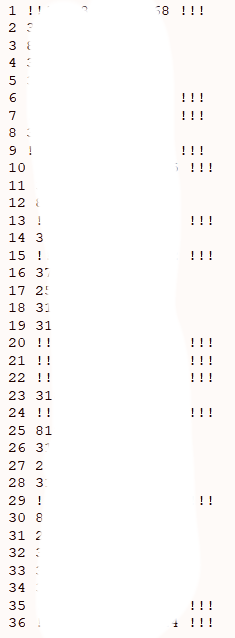
\includegraphics[height=11cm, fbox]{image2.png}
        \captionof{figure}{Das linke Bild}
        \label{fig:someotherimage}
    \end{minipage}
    \hfill
    \begin{minipage}[b]{0.4\textwidth}
        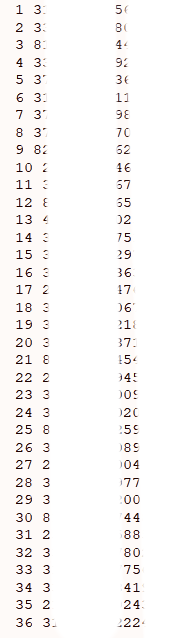
\includegraphics[height=11cm, fbox]{image1.png}
        \captionof{figure}{Das rechte Bild}
        \label{fig:yetanotherimage}
    \end{minipage}
\endminipage\par\medskip



